\documentclass[11pt]{article}
\usepackage{xcolor}
\usepackage{listings}
\usepackage{graphicx}
\usepackage{url}
\usepackage{multicol}
\usepackage{verbatim}
\usepackage{listings}
\usepackage{placeins}
\usepackage{hyperref} % Required for hyperlinks
% Define a custom color for the terminal command
\definecolor{terminalcolor}{RGB}{0, 128, 0}

\hypersetup{
    colorlinks=true,
    linkcolor=black,
    urlcolor=green
}

% Define a custom command for highlighting terminal commands
\newcommand{\labNo}{5}
\newcommand{\labTitle}{Implementation of flow control and reliable data transfer through management of
timeout, fast retransmit, cumulative acknowledgment, loss of data and acknowledgment packets.}

\begin{document}

\begin{titlepage}
    \begin{center}
        
\includegraphics[scale=0.35]{du_logo.png}\par
        \begin{Huge}
            \textsc{University of Dhaka}\par
        \end{Huge}
        \begin{Large}
            Department of Computer Science and Engineering\par \vspace{1cm}
            CSE-3111 : Computer Networking Lab \\[12pt]    
            Lab Report \labNo : \labTitle
        \end{Large}
    \end{center}
    
    \vfill
    
    \begin{large}
        \begin{multicols}{2}
            \textbf{Submitted By :\\[12pt]}
                Name: Md. Emon Khan\\[8pt]
                Roll No : 30\\[12pt]
                Name: Mahmudul Hasan\\[8pt]
                Roll No : 60\\[12pt]
                
            \columnbreak
            
            \noindent
            \textbf{Submitted To :\\[12pt]}
                Dr. Md. Abdur Razzaque\\[12pt]
                Dr. Md. Mamun Or Rashid\\[12pt]
                Dr. Muhammad Ibrahim\\[12pt]
                Md. Redwan Ahmed Rizvee
        \end{multicols}
    \end{large} 
    
\textbf{Submitted On :} \today\\[20pt]

\end{titlepage}
\tableofcontents
\newpage
\section{Introduction}
The primary goal of Lab-5 is to investigate flow control and learn about the reliable data transfer mechanism. The experiment focuses on two key tasks: TCP flow control and reliable data transfer. In Task 1, we configure the server to implement TCP flow control by setting the receive window size, which dictates the amount of data the receiver can accept before sending an acknowledgment. Clients are configured to utilize Cumulative Acknowledgment, where the receiver sends acknowledgments for the highest sequence number received, ensuring the orderly reception of data packets. In Task 2, we calculate SampleRTT values and utilize the Exponentially Weighted Moving Average (EWMA) equation to estimate Round-Trip Time (RTT) and calculate retransmission timeouts (RTO). Finally, we analyze the captured network traffic to evaluate the performance of TCP flow control.
\subsection{Objectives}
Some of the preliminary objectives of this lab experiment are:
\begin{itemize}
   \item To gather knowledge about how TCP controls the flow of data between a sender and a receiver
   \item To learn how TCP implements reliable data transfer and cumulative acknowledgment
\end{itemize}

\section{Theory}
TCP is a transport layer protocol that provides reliable, ordered, and error-checked delivery of a stream of bytes between two applications running on the same network connection. TCP involves one server and one client. Before a connection is established, the server must be listening for connection requests. TCP employs a three-way handshake (active open), retransmission, and error detection mechanisms to enhance reliability. Additionally, TCP maintains various operations to establish perfect communication between the server and client, including connection management, error detection, error recovery, congestion control, connection termination, flow control, etc.

There are mainly two types of TCP flow control: feedback-based control and rate-based flow control.

In feedback-based flow control, there are mainly two protocols: sliding window and stop-and-wait protocol.
\subsection{Flow Control}
Flow control is a process that regulates the data transmission rate between two nodes (Sender and Receiver). If the sender's data transmission rate is faster than the receiving rate, the receiver may be unable to get and process data. This situation arises due to high traffic load and low processing power. Flow control ensures that a sender does not overwhelm a receiver with too much data too quickly. The goal of flow control is to prevent buffer overflow, which can lead to dropped packets and poor network performance.

\subsection{Congestion Control}
Congestion occurs when a sender sends too much data over a network, which means there is an availability of many packets in the network. As a result, the network becomes overloaded, leading to dropped packets and poor network performance, as well as delays in packet delivery. To prevent this situation, congestion control is used. Congestion on the network may be significantly decreased by minimizing the load on the network by the transport layer. Congestion control is the responsibility of the transport and the network layer.

\section{Methodology}
\subsection{Task1: Implementaion of TCP Flow Control}
    \subsubsection{Client:}
        \begin{itemize}
            \item In the client side we create a data from a PDF file for testing
            \item We receive the window size specified by the server and then send the data dispersed into a lot of chunks consisting of different packet sequences
            \item Upon receiving each chunk of data, the server sends an acknowledgement 
            \item If the acknowledgment matches the sequence we don't need to resend
            \item If it doesn't, then we need to resend the data
            \item We send a dummy data of length 0 to tell the server that the data transmission has ended
        \end{itemize}
    \subsubsection{Server:}
        \begin{itemize}
            \item In the server side, we first specify our window size 
            \item Then we expect a sequence of data and wait for the client to send the expected sequence
            \item If the sent data is the expected sequence, then we send an acknowledgement
            \item Otherwise, we send the the acknowledgement of the last received data packet sequence
            \item Upon receiving a dummy data of 0 length, the transmission ends
        \end{itemize}

\newpage
\section{Experimental result}
Some Snapshots of the terminal output for each of these tools.
    \subsection{Task 1: Implementaion of TCP Flow Control}
    \begin{figure}[h]
        \centering
        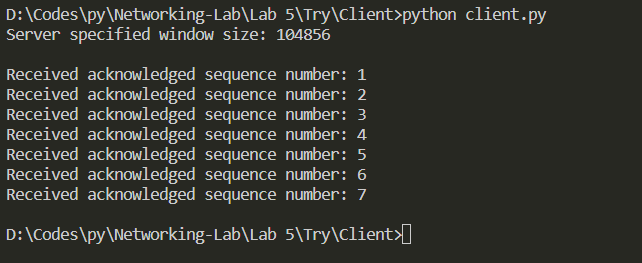
\includegraphics[width=1.0\textwidth]{client.png}
        \caption{Terminal Output for Client When Window Size is Big}
        \label{fig:response_message}
    \end{figure}
    \FloatBarrier
    \begin{figure}[h]
        \centering
        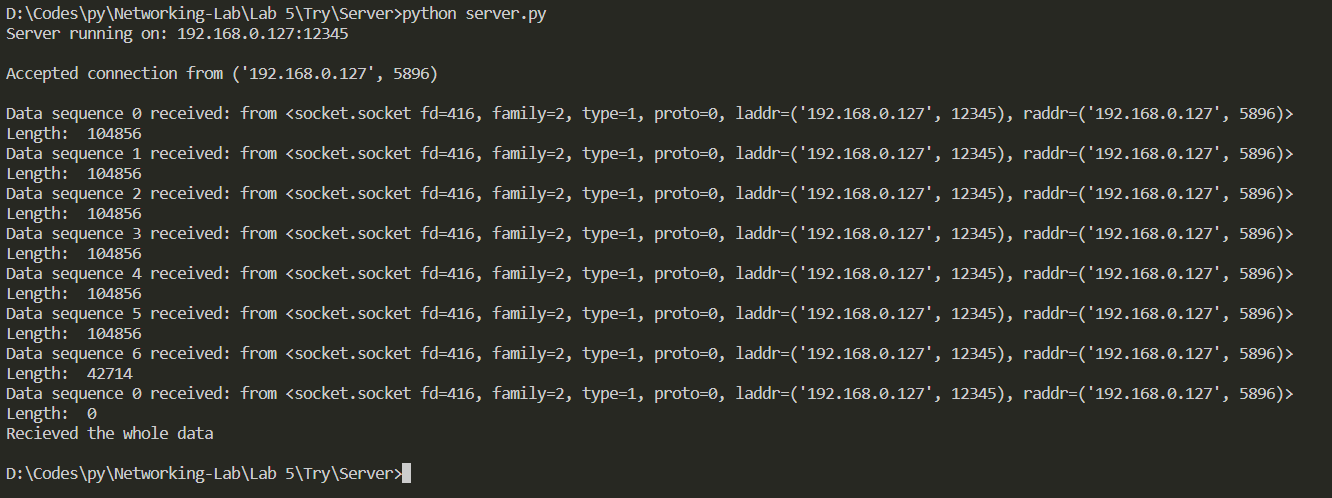
\includegraphics[width=1.0\textwidth]{server.png}
        \caption{Terminal Output for Server When Window Size is Big}
        \label{fig:response_message}
    \end{figure}
    \FloatBarrier
    \begin{figure}[h]
        \centering
        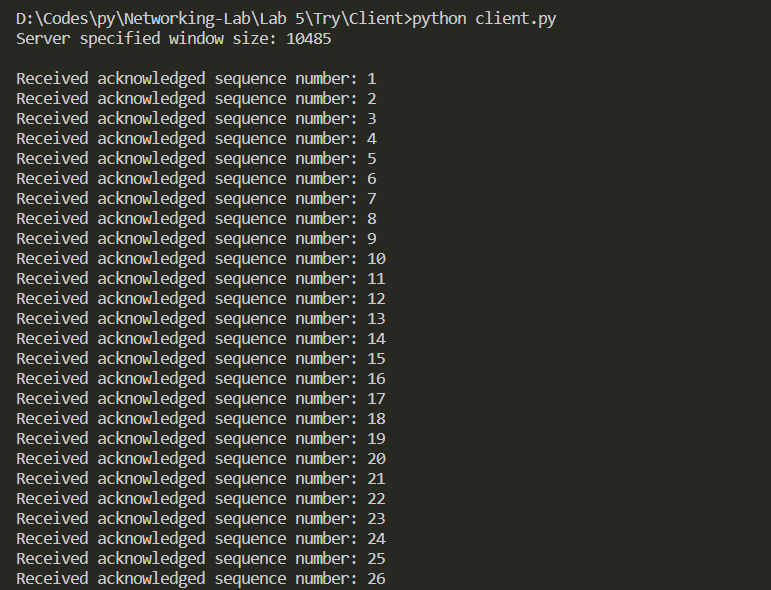
\includegraphics[width=1.0\textwidth]{client2.png}
        \caption{Terminal Output for Client When Window Size is Small}
        \label{fig:response_message}
    \end{figure}
    \FloatBarrier
    \begin{figure}[h]
        \centering
        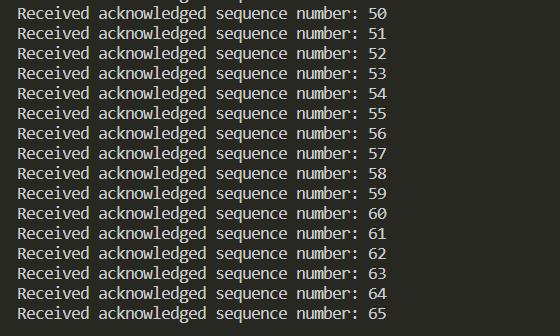
\includegraphics[width=1.0\textwidth]{client2.2.png}
        \caption{Terminal Output for Client When Window Size is Small}
    \end{figure}
    \FloatBarrier
    
    \begin{figure}[h]
        \centering
        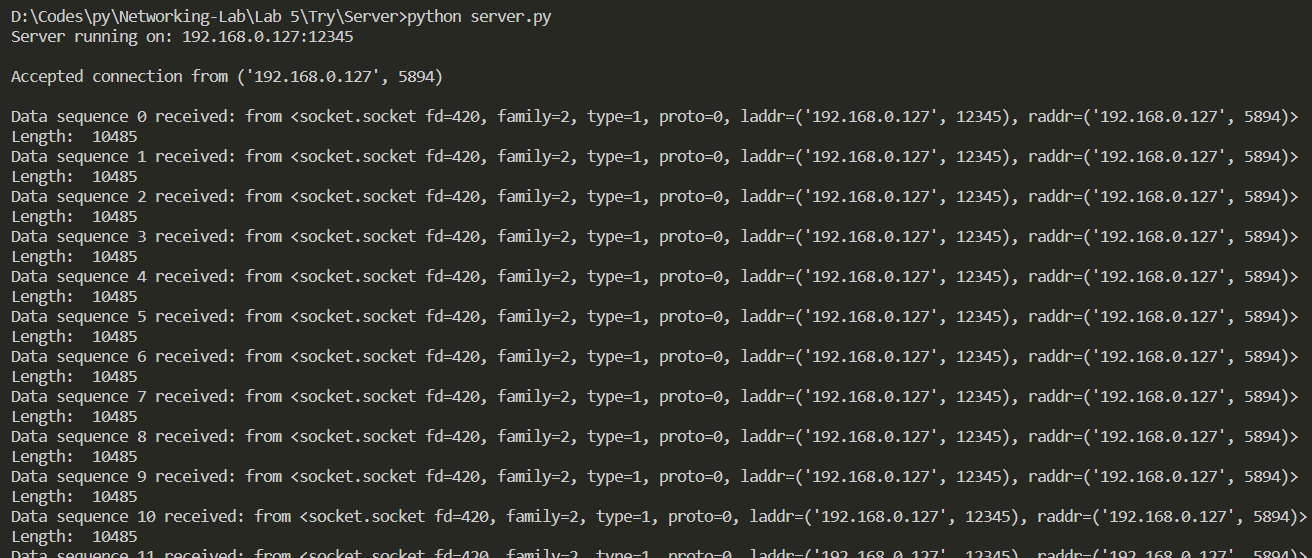
\includegraphics[width=1.0\textwidth]{server2.png}
        \caption{Terminal Output for Server When Window Size is Small}
        \label{fig:response_message}
    \end{figure}
    \FloatBarrier
    \begin{figure}[h]
        \centering
        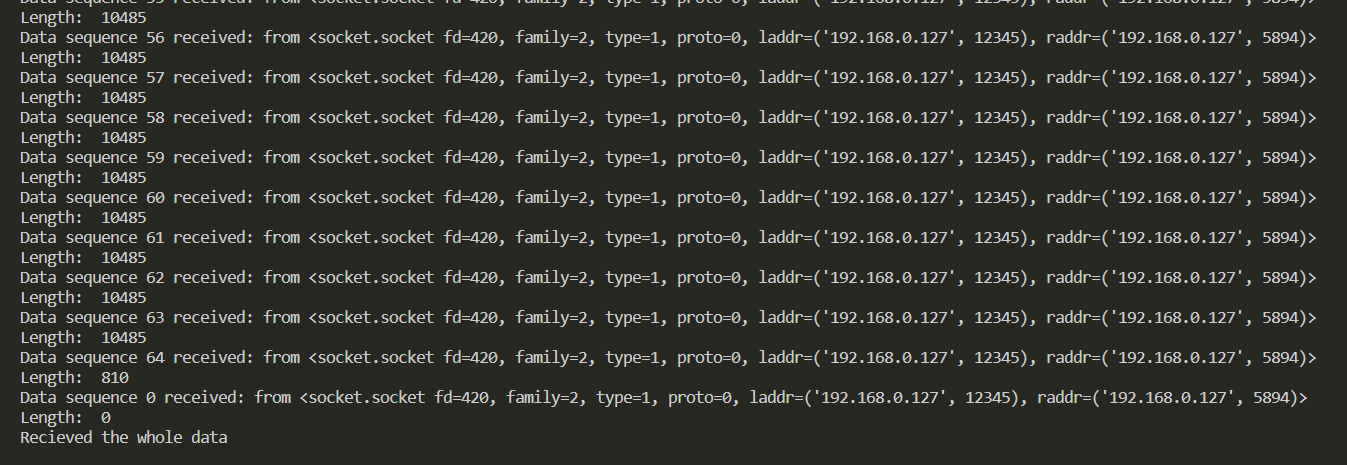
\includegraphics[width=1.0\textwidth]{server2.2.png}
        \caption{Terminal Output for Server When Window Size is Small}
        \label{fig:response_message}
    \end{figure}
    \FloatBarrier
\newpage

\section{Experience}
    \begin{itemize}
        \item Learned how TCP regulates the flow of data between sender and receiver, ensuring efficient utilization of network resources and preventing overwhelming the receiver with excessive data.
        \item Understand TCP's resilience in recovering from packet loss and ensuring data integrity.
        \item Deeper understanding of of TCP's operation and its implications for network performance.
        \item We had to learn the use of a new library "struct"
    \end{itemize}
\begin{thebibliography}{1}
    \bibitem{Geeksforgeeks} \url{https://www.geeksforgeeks.org/}
    \bibitem{Javapoint} \url{https://www.javatpoint.com/}
\end{thebibliography}

\end{document}
